\chapter{Аутентификация и Авторизация}\label{chap:auth}

Аутентификация и авторизация две очень связанные, но в то же время различные концепции. Тогда как первая имеет дело с идентификацией пользователя, вторая определяет, что пользователю позволенно делать. К сожалению, поскольку для обоих терминов часто используется абревиатура "auth", эти концепции часто объединяются.

Yesod обеспечивает встроенную поддержку для нескольких сторонних систем аутентификации, таких как OpenID, BrowserID и OAuth. Это внешние системы, которым ваше приложение доверяет удостоверение личности пользователя. Также есть поддержка более привычных способов аутентификации, таких как имя пользователя/пароль или адрес почты/пароль. Первый способ гарантирует простоту как для пользователей (нет неоходимости запоминать новые пароли), так и для разработчиков (нет нужды иметь дело со всей архитектурой безопасности), в то время как второй даёт разработчику больший контроль.

Для авторизации, мы можем воспользоваться преимуществами REST и типобезопасными URL, чтобы создать простую и декларативную систему. К тому же, поскольку весь код авторизации написан на Haskell, в вашем распоряжении будет вся гибкость языка.

В этой главе мы рассмотрим, как настроить "auth" в Yesod, и обсудим некоторые плюсы и минусы различных вариантов аутентификации.

\section{Обзор}


Пакет \footnotehref{http://hackage.haskell.org/package/yesod-auth}{yesod-auth} обеспечивает унифицированный интерефейс для различных плагинов аутентификации. Единственное, что требуется от этих плагинов, так это чтобы они идентифицировали пользователя по какой-то уникальной строке. В OpenID, к примеру, это может быть фактическое значение OpenID. В BrowserID~--- это адрес электронной почты. Для HashDB (которая использует базу данных хэшированных паролей)~--- это имя пользователя.

Каждый плагин аутентификации обеспечивает свою собственную систему для входа на сайт, будь это передача токенов с внешнего сайта, или же форма входа по адресу почты/паролю. После успешного входа, плагин устанавливает значение в пользовательской сессии, определяющее его \lstinline'AuthId'. Значением этого \lstinline'AuthId' обычно является Persistent ID из таблицы, используемой для отслеживания пользователей. 

Есть несколько функций, позволяющие получить пользовательский \lstinline'AuthId', наиболее используемыми являются \lstinline'maybeAuthId', \lstinline'requireAuthId', \lstinline'maybeAuth' и \lstinline'requireAuth'. Версии с 'require' перенаправляют на страницу входа, если пользователь ещё не вошёл, а те функции, что не оканчиваются на Id, возвращают два значения: ID таблицы и значение сущности.

Поскольку хранение \lstinline'AuthId' построено на сессиях, то применимы все их правила. В частности, данные сохраняются в зашифрованом, подписаном HMAC куки, который автоматически устаревает после определенного, задаваемого в конфигурации, периода неактивности. Кроме того, поскольку не существует серверной составляющей сессий, то при выходе из системы просто удаляются данные из куки этой сессии, и, если пользователь повторно использует старое значение куки, то сессия будет считаться действительной.

С другой стороны, авторизация контролируется несколькими методами внутри класса типов \lstinline'Yesod'. Эти методы запускаются для каждого запроса, что бы определить~--- разрешить или запретить доступ, или же потребовать от пользователя войти на сайт. По умолчанию, эти методы разрешают доступ для каждого запроса. В качестве альтернативы, вы можете реализовать авторизацию способом специально для конкретного случая, вызывая \lstinline'requireAuth' и подобные ей функции в функциях обработчиках индивидуально, хотя это отрицательно отразится на преимуществах декларативной системы авторизации.

\section{Аутентифицируй меня}

Давайте сразу рассмотрим пример с аутентификацией.

\includecode{14/authentication.hs}

Начнём с объявлений маршрутов. Сперва объявим наш стандартный маршрут \lstinline'RootR', а затем определим подсайт для аутентификации. Помните, что ему нужны четыре параметра: путь к подсайту, имя маршрута, имя подсайта и функция для получения значения подсайта. Другими словами, основываясь на строке:

\begin{lstlisting}
/auth AuthR Auth getAuth
\end{lstlisting}

Нам нужно иметь функцию \lstinline'getAuth :: MyAuthSite -> Auth'. Пока мы не напишем эту функцию сами, \footnotehref{http://hackage.haskell.org/package/yesod-auth}{\lstinline'yesod-auth'} предоставляет её автоматически. Для других подсайтов (к примеру со статическими файлами), мы обеспечиваем настройки конфигурации в значении подсайта, и поэтому нам нужно определить функцию get. Для auth подсайта, мы указываем эти настройки в отдельном классе типов \lstinline'YesodAuth'.

\begin{remark}
Почему не использовать значение подсайта? Существует достаточно много настроек, которые мы бы хотели передать auth подсайту, и делать это из типа записи (record type) было бы неудобно. Также, поскольку мы хотим иметь ассоциируемый тип \lstinline'AuthId', использование класса типов будет более естественным.

С другой стороны, почему бы не использовать класс типов для всех подсайтов? У такого подхода есть минус: вы сможете иметь только один экземпляр класса на сайт, не позволяя раздавать различные группы статичных файлов с различных маршрутов. Также, если мы хотим загружать данные во время иницииализации приложения значение подсайта подойдёт лучше.
\end{remark}

Так что же именно входит в экземпляр класса \lstinline'YesodAuth'? Шесть объявлений являются обязательными:

\begin{itemize}
    \item Ассоциированный тип \lstinline'AuthId'. Это то значение которое \lstinline'yesod-auth' будет возвращать вам, когда вы будете запрашивать, вошёл ли пользователь (через \lstinline'maybeAuthId' или \lstinline'requireAuthId'). В нашем случае, мы просто используем \lstinline'Text', для сохранения необработанного идентификатора, как вы скоро увидите это будет адрес электронной почты. 

    \item \lstinline'getAuthId' получает текущий \lstinline'AuthId' из типа данных \lstinline'Creds' (credentials~--- учетные данные). Этот тип имеет три части информации: используемый способ аутентификации (в нашем случае browserid или googleemail), текущий идентификатор, и ассоциированный список с различной дополнительной информацией.

    \item \lstinline'loginDest' возвращает маршрут куда перенаправить пользователя после успешного входа.

    \item Подобно, \lstinline'logoutDest' возвращает маршрут для перенаправления после выхода. 

    \item \lstinline'authPlugins' это список используемых способов аутентификации. В нашем примере, мы используем BrowserID, который входит через систему Mozilla BrowserID, и Google Email, который аутентифицирует почтовый адрес пользователя, используя его Google аккаунт. Что хорошо в этих двух способах, так это то, что:
    
    \begin{itemize}
        \item Они не требуют установки, в отличие от Facebook или OAuth, которые требуют задания учетных данных.
        
        \item Они используют в качестве идентификатор адрес электронной почты, который более понятен людям, в отличие от OpenID, который использует URL. 
    \end{itemize}
    
    \item \lstinline'authHttpManager' получает менеджер HTTP соединений из основного типа. Это позволяет системам аутентификации, которые использует HTTP соединения (то есть почти всем сторонним системам входа), использовать эти соединения повторно, избегая стоимости установки нового TCP подключения для каждого запроса.
\end{itemize}

Наш обработчик \lstinline'RootR', содержит ссылки на страницы входа и выхода, которые показываются в зависимости от того вошёл ли пользователь на сайт или нет. Обратите внимание, как мы конструируем эти ссылки на подсайт: первым идёт имя маршрута подсайта (\lstinline'AuthR'), следом маршрут в подсайте (\lstinline'LoginR' и \lstinline'LogoutR').

Илюстрации ниже показывает процесс входа со стороны пользователя.

\begin{figure}[h!]
  \centering
  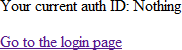
\includegraphics[width=0.4\textwidth]{14-initial-screen.png}
  \caption{Начальная загрузка страницы}
\end{figure}

\begin{figure}[h!]
  \centering
  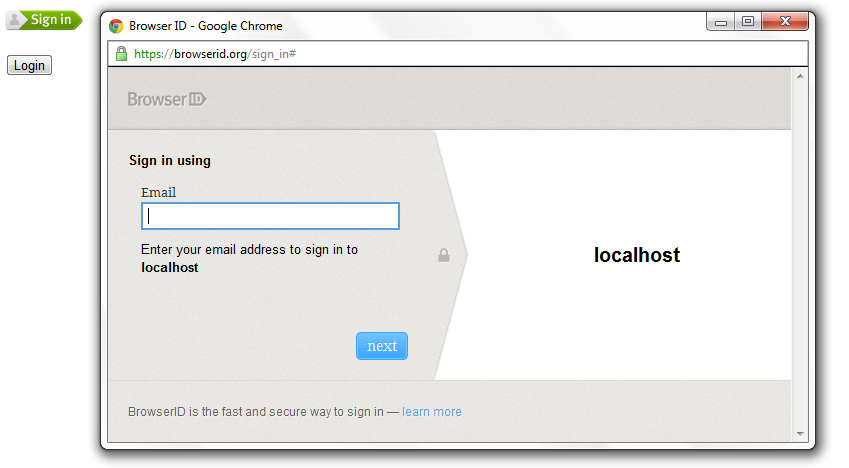
\includegraphics[width=1\textwidth]{14-login-with-browserid.png}
  \caption{Экран входа с помощью BrowserID}
\end{figure}

\begin{figure}[h!]
  \centering
  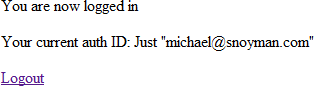
\includegraphics[width=0.6\textwidth]{14-after-login.png}
  \caption{Домащняя страница после входа}
\end{figure}

\section{Электронная почта}

Для большинства случаев будет достаточно аутентификации по адресу электронной почты, осуществляемой сервисом третьей стороны. Но иногда вам может понадобиться, чтобы пользователи использовали пароль для вашего сайта. Сгенерированый сайт не включает этой функциональности, потому что:

\begin{itemize}
    \item Чтобы безопасно использовать пароль, надо ипользовать SSL. Многие пользователи не предоставляют доступ к сайту по SSL.

    \item Несмотря на то, что система аутентификации по адресу электронной почты должным образом хранит пароли (с использованием хэширования и ``соли''), скомпрометировнная база данных всё равно может быть проблемой. Мы не делаем никаких предположений, что пользователи Yesod используют безопасные методы развёртывания.

    \item Вам нужна работающая система для отправки электронной почты. Много веб-серверов в наши дни не имеют достаточных средств для защиты от спама по сравнению с тем, что используют почтовые сервера.

    \begin{remark}
    Пример ниже использует системную программу для отправки писем~--- sendmail. Если вы хотите избежать хлопот работая с серверами электронной почты самостоятельно, вы можете использовать Amazon SES. Есть пакет \footnotehref{http://hackage.haskell.org/package/mime-mail-ses}{mime-mail-ses}, который предоставляет альтернативу использованию sendmail. Этот подход мы используем на сайте Haskellers.com.
    \end{remark}
\end{itemize}

Допустим, что вам понадобилось иметь вход с паролем специфичным для вашего сайта. Для этого Yesod предоставляет встроенную систему аутентификации. Для её использования от вас потребуется немного больше кода, ведь будет необходимо безопасно сохраненять пароли в базе данных, и отправлять пользователю почтовые сообщения (проверка аккаунта, восстановление пароля, и т.д.).

Давайте посмотрим на сайт, предоставляющий аутентификацию по адресу электронной почты и паролю и хранящий пароли в Persistent базе данных SQLite.

\includecode{14/email-authentication.hs}

\section{Авторизация}
%TOCONTINUE
Как только вы аутентифицировали пользователей, вы можете использовать их учётные данные для \emph{авторизации} дальнейших запросов. Авторизация в Yesod проста и декларативна: в большинстве случаев всего лишь необходимо добавить методы \lstinline'authRoute' и \lstinline'isAuthorized' в ваш экземпляр класса типов Yesod. Давайте рассмотрим пример:

\includecode{14/authorization.hs}

\lstinline'authRoute' должен быть вашей страницей входа, почти всегда это будет \lstinline'AuthR LoginR'. Функция \lstinline'isAuthorized' имеет два параметра: запрашиваемый маршрут, и является ли или нет запрос запросом на запись. На самом деле вы можете переопроеделить, что является запросом на запись, используя метод \lstinline'isWriteRequest', но из коробки мы следуем принципам RESTful: все запросы кроме \lstinline'GET', \lstinline'HEAD', \lstinline'OPTIONS' или \lstinline'TRACE' -- это запросы на запись.

В теле \lstinline'isAuthorized' вы можете исполнять любой \lstinline'Handler' код, какой только вы захотите, что очень удобно. Это означает, что вы можете:

\begin{itemize}
    \item обращаться к файловой системе (обычный ввод/вывод);

    \item делать запросы к базе данных;

    \item получать любые параметры сессии или запроса.
\end{itemize}

Используя эти техники, вы можете разработать настолько сложную систему авторизации, насколько захотите, или даже привязаться к уже существующей системе, используемой в вашей организации.

\section{Выводы}

Эта глава рассматривает основы настройки аутентификации пользователей, и то, как встроенные функции авторизации предоставляют простой и декларативный механизм для пользователей. Таким образом, несмотря на то, что это и сложные концепции, со многими подходами, Yesod предоставляет вам все строительные блоки, которые вам понадобятся для создания решения задач аутентификации и авторизации, соответствующего вашим требованиям.
